Il D\&C ''non funziona'' perchè ci sono molti sottoproblemi ripetuti.
\paragraph{Esempio}
\begin{flalign*}
	& X = \angleset{a,b,c,d,e} & \\
	& Y = \angleset{b,c,a,b,e} &
\end{flalign*}
Trova $LCS(X,Y)$
\bigskip

Albero delle chiamate:
\begin{center}
	\begin{tikzpicture}
	[level/.style={level distance=20mm, sibling distance=40mm/(#1-0.99)}]
	\node (a) {$(5,5)$}
	child {node (b) {$(4,4)$}
		child {node (c) {$(3,4)$}
			child {node (e) {$(2,4)$}}
			child {node (f) {$(3,3)$}}
		}
		child {node (d) {$(4,3)$}
			child {node (g) {$(3,3)$}}
			child {node (h) {$(4,2)$}}
		}
	};
	\path (a.south) -- (b.north) node [midway,right] {$e = e$};
	\node [below=5mm of b] {$b \neq d$};
	\node [below=5mm of c] {$c \neq b$};
	\node [below=5mm of d] {$d \neq a$};
	\end{tikzpicture}
\end{center}
L'istanza $(3,3)$ è ripetuta.

\paragraph{Complessità Strategia Ricorsiva}
Modello di costo: confronto tra caratteri.
\begin{flalign*}
	& T(n,m) = \begin{cases}
		0 & \text{se } n = 0 \text{ o } m = 0 \\
		T(n-1,m) + T(n,m-1) + 1 & \text{se } n,m > 0 
	\end{cases} &
\end{flalign*}
Si dimostra che
\begin{gather*}
	T(n,m) = \Theta \left(\binom{m}{n} \right) \\
	\binom{m}{2} \geq \binom{m}{2}^n 
\end{gather*}
Caso $m = 2n$
$$\binom{m}{2}^n = 2^n$$
\subsubsection{Ricorrenza sui Costi}
La scrittura della ricorrenza sui costi è il secondo passo per costruire un algoritmo di programmazione dinamica.
\bigskip

\noindent Definisco
\begin{flalign*}
	& l(i,j) = \abs{LCS(X_i,Y_j)} & \\
	& l(i,j) =
	\renewcommand{\arraystretch}{1.2}
	\left\{\begin{array}{lll}
	0 & \text{se } i = 0 \text{ o } j = 0 & \text{(caso \ref{lcs:0})} \\
	l(i-1,j-1) + 1 & \text{se } i,j > 0 \text{ e } x_i=x_j & \text{(caso \ref{lcs:1})} \\
	\max\{l(i,j-1),l(i-1,j)\} & \text{se } i,j > 0 \text{ e } x_i \neq x_j & \text{(caso \ref{lcs:2})}
	\end{array}\right. &
\end{flalign*}
Alla fine ci interessa calcolare $l(m,n)$. \par
Per calcolare $l(i,j)$ mi possono servire tre valori:
\begin{gather*}
	L = 
	\setlength{\arraycolsep}{0pt}
	\left[\begin{array}{ccccc}
	\qquad & & & & \qquad \\
	& (i{-}1,j{-}1) & & (i{-}1,j) & \\
	& & \nwarrow & \uparrow & \\
	& (i,j{-}1) & \leftarrow & (i,j) & \\
	& & & &
	\end{array}\right]
\end{gather*}
Scansione ''row-major'': riempio la tabella per righe, da sinistra a destra.
\bigskip

Informazione addizionale per costruire la sequenza (vera e propria):
\begin{flalign*}
	& b(i,j) = \begin{cases}
		\textnormal{\textquotesingle}\nwarrow\textnormal{\textquotesingle} & \text{se } x_i = y_j \\
		\textnormal{\textquotesingle}\leftarrow\textnormal{\textquotesingle} & \text{se } x_i \neq x_j \text{ e } max = LCS(i,j-1) \\
		\textnormal{\textquotesingle}\uparrow\textnormal{\textquotesingle} & \text{se } x_i \neq y_j \text{ e } max = LCS(i-1,j)
	\end{cases} &
\end{flalign*}
\pagebreak
\paragraph{Pseudocodice}
\begin{codebox}
\Procname{$\proc{LCS}(X,Y)$}
\li $m \gets \attrib{X}[length]$
\li $n \gets \attrib{Y}{length}$
\li \For $i \gets 0$ \To $m$
\li \Do
		$L[i,0] \gets 0$
	\End
\li \For $j \gets 0$ \To $n$
\li \Do
		$L[0,j] \gets 0$
	\End
\li \For $i \gets 1$ \To $m$
\li \Do
		\For $j = 1$ \To $n$
\li 	\Do
			\If $x_i = y_j$
\li 		\Then
				$L[i,j] \gets L[i-1,j-1] + 1$
\li				$B[i,j] \gets \textnormal{\textquotesingle}\nwarrow\textnormal{\textquotesingle}$
\li			\ElseIf $L[i-1,j] \geq L[i,j-1]$
\li			\Then
				$L[i,j] \gets L[i-1,j]$
\li				$B[i,j] \gets \textnormal{\textquotesingle}\uparrow\textnormal{\textquotesingle}$
\li			\ElseNoIf
\li				$L[i,j] = L[i,j-1]$
\li				$B[i,j] = \textnormal{\textquotesingle}\leftarrow\textnormal{\textquotesingle}$
			\End
		\End
	\End
\li \Return $(L[m,n],B)$
\end{codebox}
\paragraph{Complessità}
\begin{flalign*}
	& T(m,n) = \Theta(m \cdot n) & \\
	& \text{Caso } m = n \Rightarrow T(m,n) = \Theta(n^2) &
\end{flalign*}

Procedura per stampare la LCS:
\begin{codebox}
\Procname{$\proc{PrintLCS}(B,X,i,j)$}
\li \If $i = 0$ \kw{ or } $j = 0$
\li \Then \Return $\varepsilon$
	\End
\li \If $B[i,j] = \textnormal{\textquotesingle}\nwarrow\textnormal{\textquotesingle}$
\li	\Then
		 $\proc{PrintLCS}(B,X,i-1,j-1)$
\li      $\proc{Print}(x_i)$
\li \ElseIf $B[i,j] = \textnormal{\textquotesingle}\leftarrow\textnormal{\textquotesingle}$
\li \Then $\proc{PrintLCS}(B,X,i,j-1)$
\li \ElseNoIf \Comment $B[i,j] = \textnormal{\textquotesingle}\uparrow\textnormal{\textquotesingle}$
\li 	$\proc{PrintLCS}(B,X,i-1,j)$
	\End
\end{codebox}
\paragraph{Complessità} $\Theta(m) = \Theta(\abs{LCS})$

\paragraph{Esercizio}
\begin{flalign*}
	& X = \angleset{b,d,c,d} & \\
	& Y = \angleset{a,b,c,b,d} &
\end{flalign*}
Restituisci $LCS(X,Y)$ e $\abs{LCS(X,Y)}$
\begin{align*}
	& L =
	\begin{blockarray}{ccccccc}
	  &   & a & b & c & b & d \\
	\begin{block}{c[cccccc]}
	  & 0 & 0 & 0 & 0 & 0 & 0 \\
	b & 0 & 0 & \boldsymbol{1} & 1 & 1 & 1 \\
	d & 0 & 0 & 1 & 1 & 1 & 2 \\
	c & 0 & 0 & 1 & \boldsymbol{2} & 2 & 2 \\
	d & 0 & 0 & 1 & 2 & 2 & \boldsymbol{3} \\
	\end{block}
	\end{blockarray}
	& B =
	\begin{blockarray}{ccccccc}
	&   & a & b & c & b & d \\
	\begin{block}{c[cccccc]}
	  & & & & & & \\
	b & & \uparrow & \nwarrow & \leftarrow & \nwarrow & \leftarrow \\
	d & & \uparrow & \uparrow & \uparrow & \uparrow & \nwarrow \\
	c & & \uparrow & \uparrow & \nwarrow & \leftarrow & \uparrow \\
	d & & \uparrow & \uparrow & \uparrow & \uparrow & \nwarrow \\
	\end{block}
	\end{blockarray}
\end{align*}
$LCS(X,Y) = \angleset{b,c,d} \qquad \abs{LCS(X,Y)} = 3$

\paragraph{Pseudocodice Memoizzato}
\begin{codebox}
\Procname{$\proc{Init-LCS}(X,Y)$}
\li $m \gets \attrib{X}{length}$
\li $n \gets \attrib{Y}{length}$
\li \If $(m = 0)$ \kw{ or } $(n = 0)$
\li \Then \Return $0$
	\End
\li \For $i \gets 0 \To m$
\li \Do $L[i,0] \gets 0$
	\End
\li \For $j \gets 0 \To n$
\li \Do $L[0,j] \gets 0$
	\End
\li \For $i \gets 1 \To m$
\li \Do \For $i \gets 1 \To n$
\li 	\Do $L[i,j] \gets -1$
		\End
	\End
\li \Return $\proc{R-LCS}(X,Y,m,n)$
\end{codebox}
\begin{codebox}
\Procname{$\proc{R-LCS}(X,Y,i,j)$}
\li \If $L[i,j] = -1$
\li \Then
		\If $x_i = y_j$
\li 	\Then
			$L[i,j] \gets \proc{R-LCS}(X,Y,i-1,j-1)$
\li		\ElseIf $\proc{R-LCS}(X,Y,i-1,j) \geq \proc{R-LCS}(X,Y,i,j-1)$
\li		\Then
			$L[i,j] \gets L[i-1,j]$
\li		\ElseNoIf
\li			$L[i,j] \gets L[i,j-1]$
		\End
	\End
\li \Return $L[i,j]$
\end{codebox}
\paragraph{Complessità} $O(m \cdot n)$

\paragraph{Osservazione}
Se $x_i = y_j$ sempre, invoco \texttt{R-LCS(X,Y,i-1,j-1)} ma non invoco mai \texttt{R-LCS(X,Y,i-1,j)} o \texttt{R-LCS(X,Y,i,j-1)}.
\bigskip

Ad esempio
\begin{flalign*}
	& X = \angleset{a,a,b,b,c} & \\
	& Y = \angleset{b,b,c}
\end{flalign*}
Albero delle chiamate:
\begin{center}
	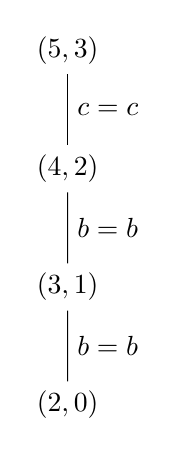
\begin{tikzpicture}
	\node (a) {$(5,3)$}
	child {node (b) {$(4,2)$}
		child {node (c) {$(3,1)$}
			child {node (d) {$(2,0)$}}
		}
	};
	\path (a.south) -- (b.north) node [midway,right] {$c = c$};
	\path (b.south) -- (c.north) node [midway,right] {$b = b$};
	\path (c.south) -- (d.north) node [midway,right] {$b = b$};
	\end{tikzpicture}
\end{center}
In generale, se $Y$ è suffisso di $n \leq m$ caratteri di $X$, la complessità di \texttt{R-LCS} nel caso migliore è:
$$T_{R-LCS}(m,n) = n$$
Inoltre,
\begin{gather*}
	\Omega_{LCS}(m+n) \approxeq \Omega(n) \\
	O_{LCS,R-LCS}(m \cdot n) \approxeq O(n^2)
\end{gather*}

\paragraph{Spazio}
$$S_{LCS}(m,n) = \Theta(m,n)$$
Tuttavia, posso migliorarlo a
$$\Theta(2n) = \Theta(n)$$
poichè mi bastano due righe della tabella in memoria ad ogni istante, quindi due vettori lunghi $n$. \par
Inoltre, se $m \ll n$, posso fare un'ulteriore ottimizzazione utilizzando la tecnica ''column-major'', cioè scansione per colonne, con due vettori lunghi $m$.